\documentclass{beamer}
\usetheme{Rochester}
\usepackage{tcolorbox}
\tcbuselibrary{listings}
\usepackage{inconsolata}

\geometry{paperwidth = 4.75in, paperheight = 4.75in}

% Custom U of C color palette
\definecolor{ucMaroon}{RGB}{128,0,0}
\definecolor{ucDarkGray}{RGB}{118,118,118}
\definecolor{ucLightGray}{RGB}{214,214,206}

\setbeamercolor{block title}{fg=white,bg=ucMaroon}
\setbeamercolor{block title alerted}{use=alerted text,fg=white,bg=alerted text.fg}
\setbeamercolor{block title example}{use=example text,fg=white,bg=example text.fg}
\setbeamercolor{block body}{parent=normal text,use=block title,bg=ucLightGray}
\setbeamercolor{block body alerted}{parent=normal text,use=block title alerted,bg=block title alerted.bg}
\setbeamercolor{block body example}{parent=normal text,use=block title example,bg=block title example.bg}

\setbeamercolor{palette primary}{fg=white,bg=ucMaroon}
\setbeamercolor{palette secondary}{fg=white,bg=ucLightGray}
\setbeamercolor{palette tertiary}{fg=white,bg=ucDarkGray}
\setbeamercolor{palette quaternary}{fg=white,bg=black}

\setbeamercolor{sidebar}{bg=ucMaroon}

\setbeamercolor{palette sidebar primary}{fg=ucMaroon}
\setbeamercolor{palette sidebar secondary}{fg=white}
\setbeamercolor{palette sidebar tertiary}{fg=ucMaroon}
\setbeamercolor{palette sidebar quaternary}{fg=white}

\setbeamercolor{titlelike}{parent=palette primary}
\setbeamercolor{itemize item}{fg=ucMaroon}

% Code block formatting. Fragile frames needed for these to work.
\newtcblisting{gitCommand}{
  colframe=black,
  colback=ucLightGray,
  boxrule=1pt,
  arc=2pt,
  left=6pt,
  right=6pt,
  top=6pt,
  bottom=6pt,
  before=\vspace{6pt},
  boxsep=0pt,
  listing only,
  hbox
}


\title{Intermediate Git}
\subtitle{Day 3: Branching and Merging}
\author{Raman A.~Shah}
\date{}

\begin{document}

%% Title
\begin{frame}[plain]
  \titlepage
  \footnotesize{Copyright (c) 2015 by Raman A.~Shah.\\
  \href{https://creativecommons.org/licenses/by-nc-sa/3.0/legalcode}
       {Creative Commons BY-NC-SA 3.0 Unported}.\\
   \href{https://github.com/ramanshah/intermediate\_git}
        {https://github.com/ramanshah/intermediate\_git}}
\end{frame}

%% Commits point to commits
\begin{frame}{Commits point to commits}
  \begin{figure}
    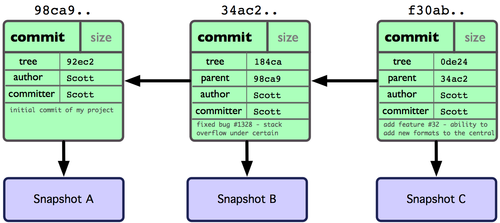
\includegraphics[scale=0.8]{18333fig0302-tn.png}
    \\ Each commit (but the first) has a parent.
  \end{figure}
  \footnotesize{Scott Chacon,
    \emph{Pro Git},
    Fig.~3-2.
    \href{https://creativecommons.org/licenses/by-nc-sa/3.0/legalcode}{CC-BY-NC-SA}.
    \href{https://progit.org/}{https://progit.org/}}
\end{frame}

%% Branches point to commits
\begin{frame}{Branches point to commits}
  \begin{figure}
    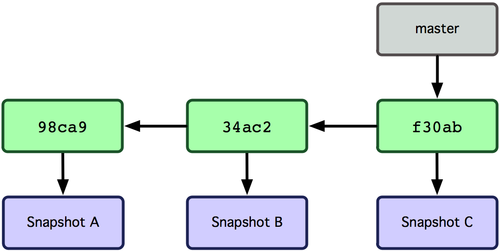
\includegraphics[scale=0.8]{18333fig0303-tn.png}
    \\ A branch is just a pointer to a commit.
  \end{figure}
  \footnotesize{Scott Chacon,
    \emph{Pro Git},
    Fig.~3-3.
    \href{https://creativecommons.org/licenses/by-nc-sa/3.0/legalcode}{CC-BY-NC-SA}.
    \href{https://progit.org/}{https://progit.org/}}
\end{frame}

%% Branches can diverge
\begin{frame}{Branches can diverge}
  \begin{figure}
    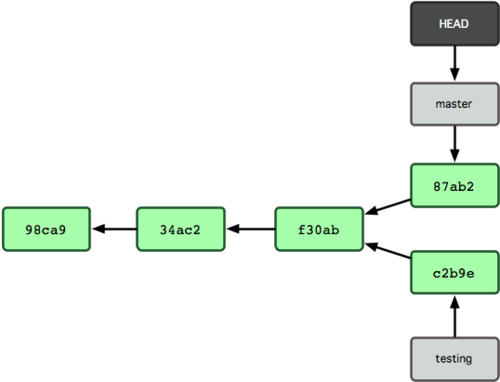
\includegraphics[scale=0.8]{18333fig0309-tn.png}
    \\ Branches enable you to develop different versions of the product concurrently.
  \end{figure}
  \footnotesize{Scott Chacon,
    \emph{Pro Git},
    Fig.~3-9.
    \href{https://creativecommons.org/licenses/by-nc-sa/3.0/legalcode}{CC-BY-NC-SA}.
    \href{https://progit.org/}{https://progit.org/}}
\end{frame}

%% Merging brings them back
\begin{frame}{Merging brings them back}
  \begin{figure}
    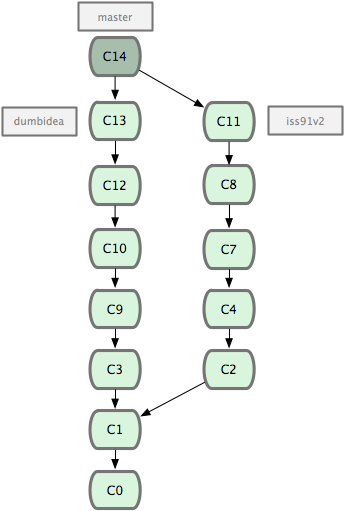
\includegraphics[scale=0.8]{18333fig0321-tn.png}
    \\ Because of merging, you can work on different aspects of a final desired product concurrently.
  \end{figure}
  \footnotesize{Scott Chacon,
    \emph{Pro Git},
    Fig.~3-21.
    \href{https://creativecommons.org/licenses/by-nc-sa/3.0/legalcode}{CC-BY-NC-SA}.
    \href{https://progit.org/}{https://progit.org/}}
\end{frame}

%% Back to the Day 2 repo
\begin{frame}[fragile]{Back to the Day 2 repo}
  Do you have a clean sample repository from last time?

  \begin{gitCommand}
cd sample
git status
  \end{gitCommand}

  If not, either clone the course repo or refresh it with
  \texttt{git pull origin master}:

  \begin{gitCommand}
git clone https://github.com/\
ramanshah/intermediate_git.git
  \end{gitCommand}

  Then decompress an updated sample repository:

  \begin{gitCommand}
cp ./intermediate_git/day3/sample.tgz .
tar xzvf sample.tgz
cd sample
git status
  \end{gitCommand}
\end{frame}

%% Your first branches
\begin{frame}[fragile]{Your first branches}

  Between each of the following, monitor with:

  \begin{gitCommand}git branch\end{gitCommand}

  \begin{gitCommand}
git branch foo
git checkout foo
git checkout master
git branch -d foo
  \end{gitCommand}
\end{frame}

%% git checkout moves HEAD
\begin{frame}{\texttt{git checkout} moves \texttt{HEAD}}
  \begin{figure}
    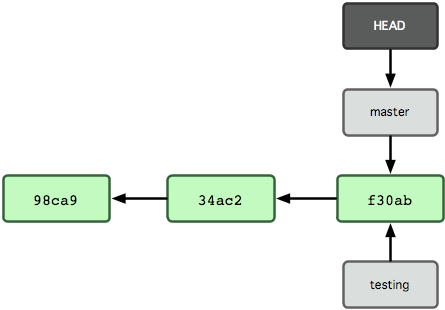
\includegraphics[scale=0.8]{18333fig0305-tn.png}
    \\ \texttt{git checkout master}
  \end{figure}
  \footnotesize{Scott Chacon,
    \emph{Pro Git},
    Fig.~3-5.
    \href{https://creativecommons.org/licenses/by-nc-sa/3.0/legalcode}{CC-BY-NC-SA}.
    \href{https://progit.org/}{https://progit.org/}}
\end{frame}

\begin{frame}{\texttt{git checkout} moves \texttt{HEAD}}
  \begin{figure}
    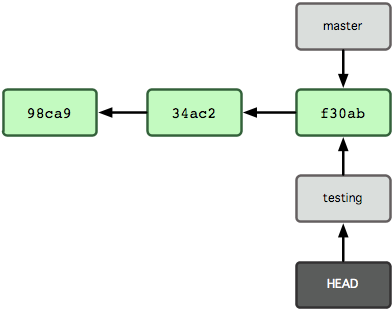
\includegraphics[scale=0.8]{18333fig0306-tn.png}
    \\ \texttt{git checkout testing}
  \end{figure}
  \footnotesize{Scott Chacon,
    \emph{Pro Git},
    Fig.~3-6.
    \href{https://creativecommons.org/licenses/by-nc-sa/3.0/legalcode}{CC-BY-NC-SA}.
    \href{https://progit.org/}{https://progit.org/}}
\end{frame}

%% Hacking on a branch
\begin{frame}[fragile]{Hacking on a branch}
  A shortcut for:

  \begin{gitCommand}
git branch experiment
git checkout experiment
  \end{gitCommand}

  is:

  \begin{gitCommand}git checkout -b experiment\end{gitCommand}

  After making some commits, you can throw away the experimental commits with:

  \begin{gitCommand}
git checkout master
git branch -D experiment
  \end{gitCommand}

\end{frame}

%% Scenario #1: clean merge
\begin{frame}{Scenario \#1: clean merge}
  In the push to complete a project, two things will happen concurrently:

  \begin{itemize}
    \item Debug an analysis code
    \item Flesh out a manuscript
  \end{itemize}
\end{frame}

%% Do work on two branches
\begin{frame}[fragile]{Do work on two branches}

  Create a branch for debugging the analysis code:

  \begin{gitCommand}git checkout -b fix_math\end{gitCommand}

  Fix the bug in \texttt{R/square.R} using R's \texttt{*} operator:

  \begin{gitCommand}
...
git commit ...
  \end{gitCommand}

  Do the work to flesh out the manuscript on \texttt{master}:

  \begin{gitCommand}git checkout master\end{gitCommand}

  Explain in \texttt{paper/paper.tex} that $ x^2 = x \times x $.

  \begin{gitCommand}
...
git commit ...
  \end{gitCommand}
\end{frame}

\begin{frame}[fragile]{Branches are lightweight}
  \begin{gitCommand}
cat .git/refs/heads/master
cat .git/refs/heads/fix_math
  \end{gitCommand}
\end{frame}

%% Git plans a three-way merge
\begin{frame}{Git plans a three-way merge}
  \begin{figure}
    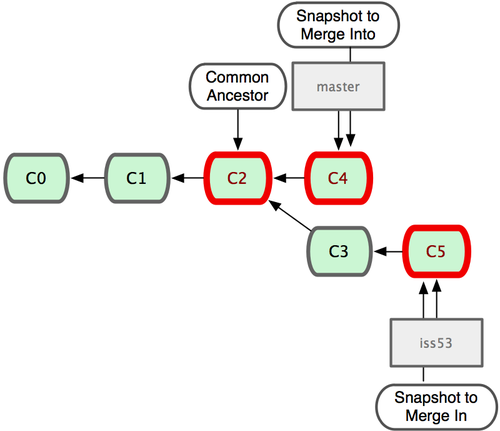
\includegraphics[scale=0.8]{18333fig0316-tn.png}
    \\ Git figures out the best common ancestor on its own\ldots
  \end{figure}
  \footnotesize{Scott Chacon,
    \emph{Pro Git},
    Fig.~3-16.
    \href{https://creativecommons.org/licenses/by-nc-sa/3.0/legalcode}{CC-BY-NC-SA}.
    \href{https://progit.org/}{https://progit.org/}}
\end{frame}

\begin{frame}{Git plans a three-way merge}
  \begin{figure}
    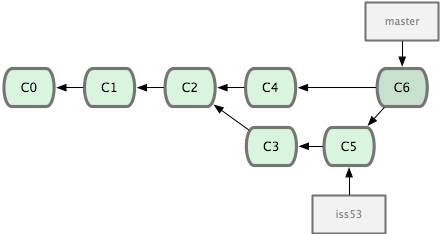
\includegraphics[scale=0.8]{18333fig0317-tn.png}
    \\ \ldots and creates a ``merge commit'' from the three relevant snapshots.
  \end{figure}
  \footnotesize{Scott Chacon,
    \emph{Pro Git},
    Fig.~3-17.
    \href{https://creativecommons.org/licenses/by-nc-sa/3.0/legalcode}{CC-BY-NC-SA}.
    \href{https://progit.org/}{https://progit.org/}}
\end{frame}

%% Merge our work
\begin{frame}[fragile]{Merge our work}
  Merge the work \emph{from} \texttt{fix\_math} \emph{into} \texttt{master}, updating \texttt{master}:

  \begin{gitCommand}
git checkout master
git merge fix_math
  \end{gitCommand}

  Behold your successful merge!

  \begin{gitCommand}git log --oneline --graph\end{gitCommand}

  Throw away your successfully merged branch:

  \begin{gitCommand}git branch -d fix_math\end{gitCommand}

  And it's gone:

  \begin{gitCommand}git branch\end{gitCommand}

\end{frame}

%% Scenario #2: merge conflict
\begin{frame}[fragile]{Scenario \#2: merge conflict}
  Let's pretend that merge never happened:

  \begin{gitCommand}
git checkout master
git reset --hard HEAD~1
  \end{gitCommand}

  And say that on \texttt{master}, we fixed the math bug in a
  different way using R's \texttt{**} operator:

  \begin{gitCommand}
...
git commit ...
  \end{gitCommand}

  Then what?

  \begin{gitCommand}git merge fix_math\end{gitCommand}
\end{frame}

%% Panic button
\begin{frame}[fragile]{Panic button}
  \begin{gitCommand}git merge --abort\end{gitCommand}
\end{frame}

%% Fixing a merge conflict
\begin{frame}[fragile]{Fixing a merge conflict}
  \begin{gitCommand}git merge fix_math\end{gitCommand}

  Have a look in the file that didn't merge cleanly. Make it look the
  way you want it to look. To tell Git that the file is ``fixed,'' you
  stage it!

  \begin{gitCommand}
...
git add R/square.R
  \end{gitCommand}

  Then commit as usual:

  \begin{gitCommand}git commit ...\end{gitCommand}

\end{frame}

%% Fast-forward merges
\begin{frame}{Fast-forward merges}
  \begin{figure}
    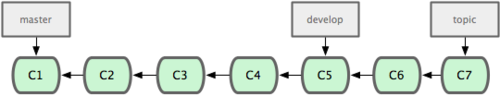
\includegraphics[scale=0.8]{18333fig0318-tn.png}
    \\ \texttt{git checkout master} followed by \texttt{git merge develop}
    just moves a pointer!
  \end{figure}
  \footnotesize{Scott Chacon,
    \emph{Pro Git},
    Fig.~3-18.
    \href{https://creativecommons.org/licenses/by-nc-sa/3.0/legalcode}{CC-BY-NC-SA}.
    \href{https://progit.org/}{https://progit.org/}}
\end{frame}

\begin{frame}{Fast-forward merges}
  \begin{figure}
    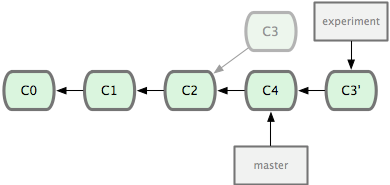
\includegraphics[scale=0.8]{18333fig0329-tn.png}
    \\ Rebasing can turn a branched history into a linear history.
  \end{figure}
  \footnotesize{Scott Chacon,
    \emph{Pro Git},
    Fig.~3-29.
    \href{https://creativecommons.org/licenses/by-nc-sa/3.0/legalcode}{CC-BY-NC-SA}.
    \href{https://progit.org/}{https://progit.org/}}
\end{frame}

%% Rewrite history: git rebase
\begin{frame}{Rewrite history: git rebase}
  \huge {
  Never modify history that someone else has seen.
  }
\end{frame}

%% Scenario #3: clean rebase
\begin{frame}[fragile]{Scenario \#3: clean rebase}
  We'll rewind to just before our merge in Scenario \#1: let's get rid
  of that merge but also the conflicting commit that we'd introduced
  on \texttt{master}:

  \begin{gitCommand}git reset --hard HEAD~2\end{gitCommand}
\end{frame}

\begin{frame}[fragile]{Scenario \#3: clean rebase}
  Replay the work \emph{from} \texttt{fix\_math} \emph{onto} the tip
  of \texttt{master}, creating a similar (but
  different) \texttt{fix\_math}:

  \begin{gitCommand}
git checkout fix_math
git rebase master
  \end{gitCommand}

  Now the merge is a fast-forward!

  \begin{gitCommand}
git checkout master
git merge fix_math
git log --oneline --graph
  \end{gitCommand}

  Throw away your successfully merged branch:

  \begin{gitCommand}git branch -d fix_math\end{gitCommand}
\end{frame}

\end{document}
